\chapter{Comparison of different eddy detection methods}\label{sec-eval}

In this chapter, we evaluate the robustness of the Lagrangian method by comparing the eddy detecting results between SSHA Eulerian method (as illustrated in figure \ref{A schematic SSHA anticyclonic eddy}) and the LAVD method.

\section{Introduction of Mesoscale Eddy Trajectory Atlas}

We download \href{https://www.aviso.altimetry.fr/en/data/products/value-added-products/global-mesoscale-eddy-trajectory-product/meta2-0-dt.html}{Eulerian eddies trajectories data}  from AVISO+, which detected eddies from Sea Level Anomaly field of merged altimetry datasets using SSHA method as described in chapter \ref{Eulerian methods} and told us information of type, speed, and radius of Eulerian eddies globally \cite{chelton2011global}. This dataset contains eddies with a life cycle of more than 4 weeks. The time frame of the dataset is from 1993 to the present. In this chapter, all the eddies in the spatial range 70°W to 30°W, 60°S to 30°S are used for the statistical analysis of Eulerian eddies. The time range of the vortex dataset selected for the study is from January 1993 to December 2019.


\section{Statistics results of Eulerian detection method}


The statistics Eulerian detection results are shown below in figure \ref{anticyclonic eddies numbers from 1993 to 2019} and figure \ref{cyclonic eddies numbers from 1993 to 2019} (we separate the research region into $1^\circ \times 1^\circ$ sub-domain and sum up the eddies appearing respectively in each sub-domain). From 1993 to 2019, 13683 eddies were generated in the whole region, 6686 of them are anti-cyclonic eddies and 6997 are cyclonic ones. Among all the eddies, along the coast of South America, only a few eddies were detected, which is consistent with Lagrangian methods. In the northern part and the southwest part of the Argentine Basin, we observe vast numbers of eddies. In the center part of the Argentine Basin, only a few eddies were detected. Many vortices have been observed in the Southern Ocean region or in the connecting water region between Argentine Basin and the Southern Ocean near the islands. The general pattern is quite similar to the results in the chapter \ref{Eddies features analysis} when the Lagrangian method is adopted although the Eulerian method could detect a higher number of eddies.

\begin{figure}[ht]
  \centering
  \setlength{\abovecaptionskip}{0.cm}
  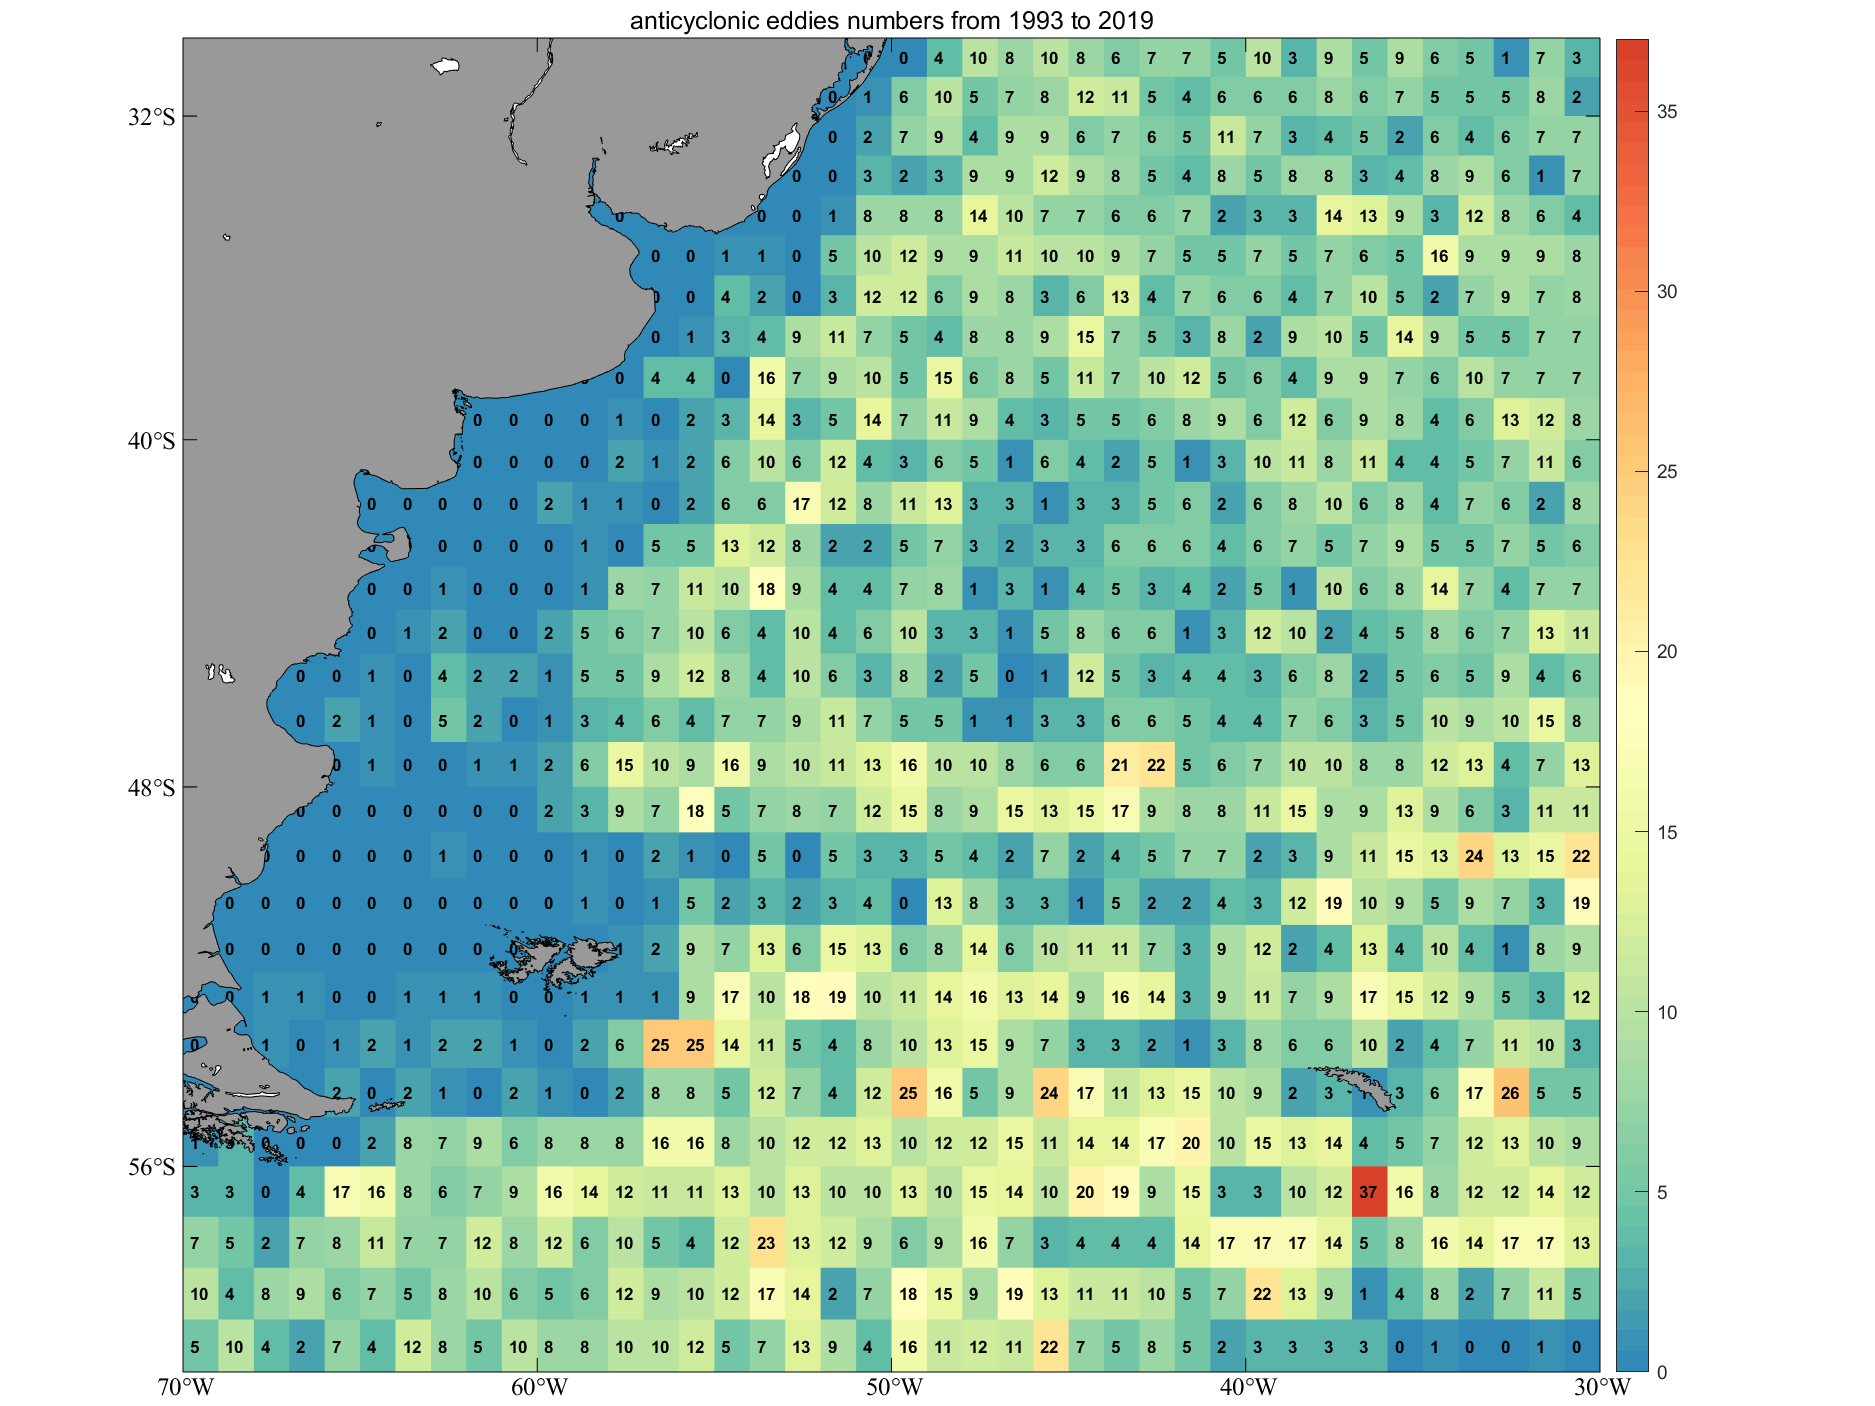
\includegraphics[width=15cm]{chapter/figure/anticyclonic eddies numbers from 1993 to 2019.png}
  \caption
  {Anticyclonic eddies numbers from 1993 to 2019}
  \label{anticyclonic eddies numbers from 1993 to 2019}
\end{figure}

\begin{figure}[ht]
  \centering
  \setlength{\abovecaptionskip}{0.cm}
  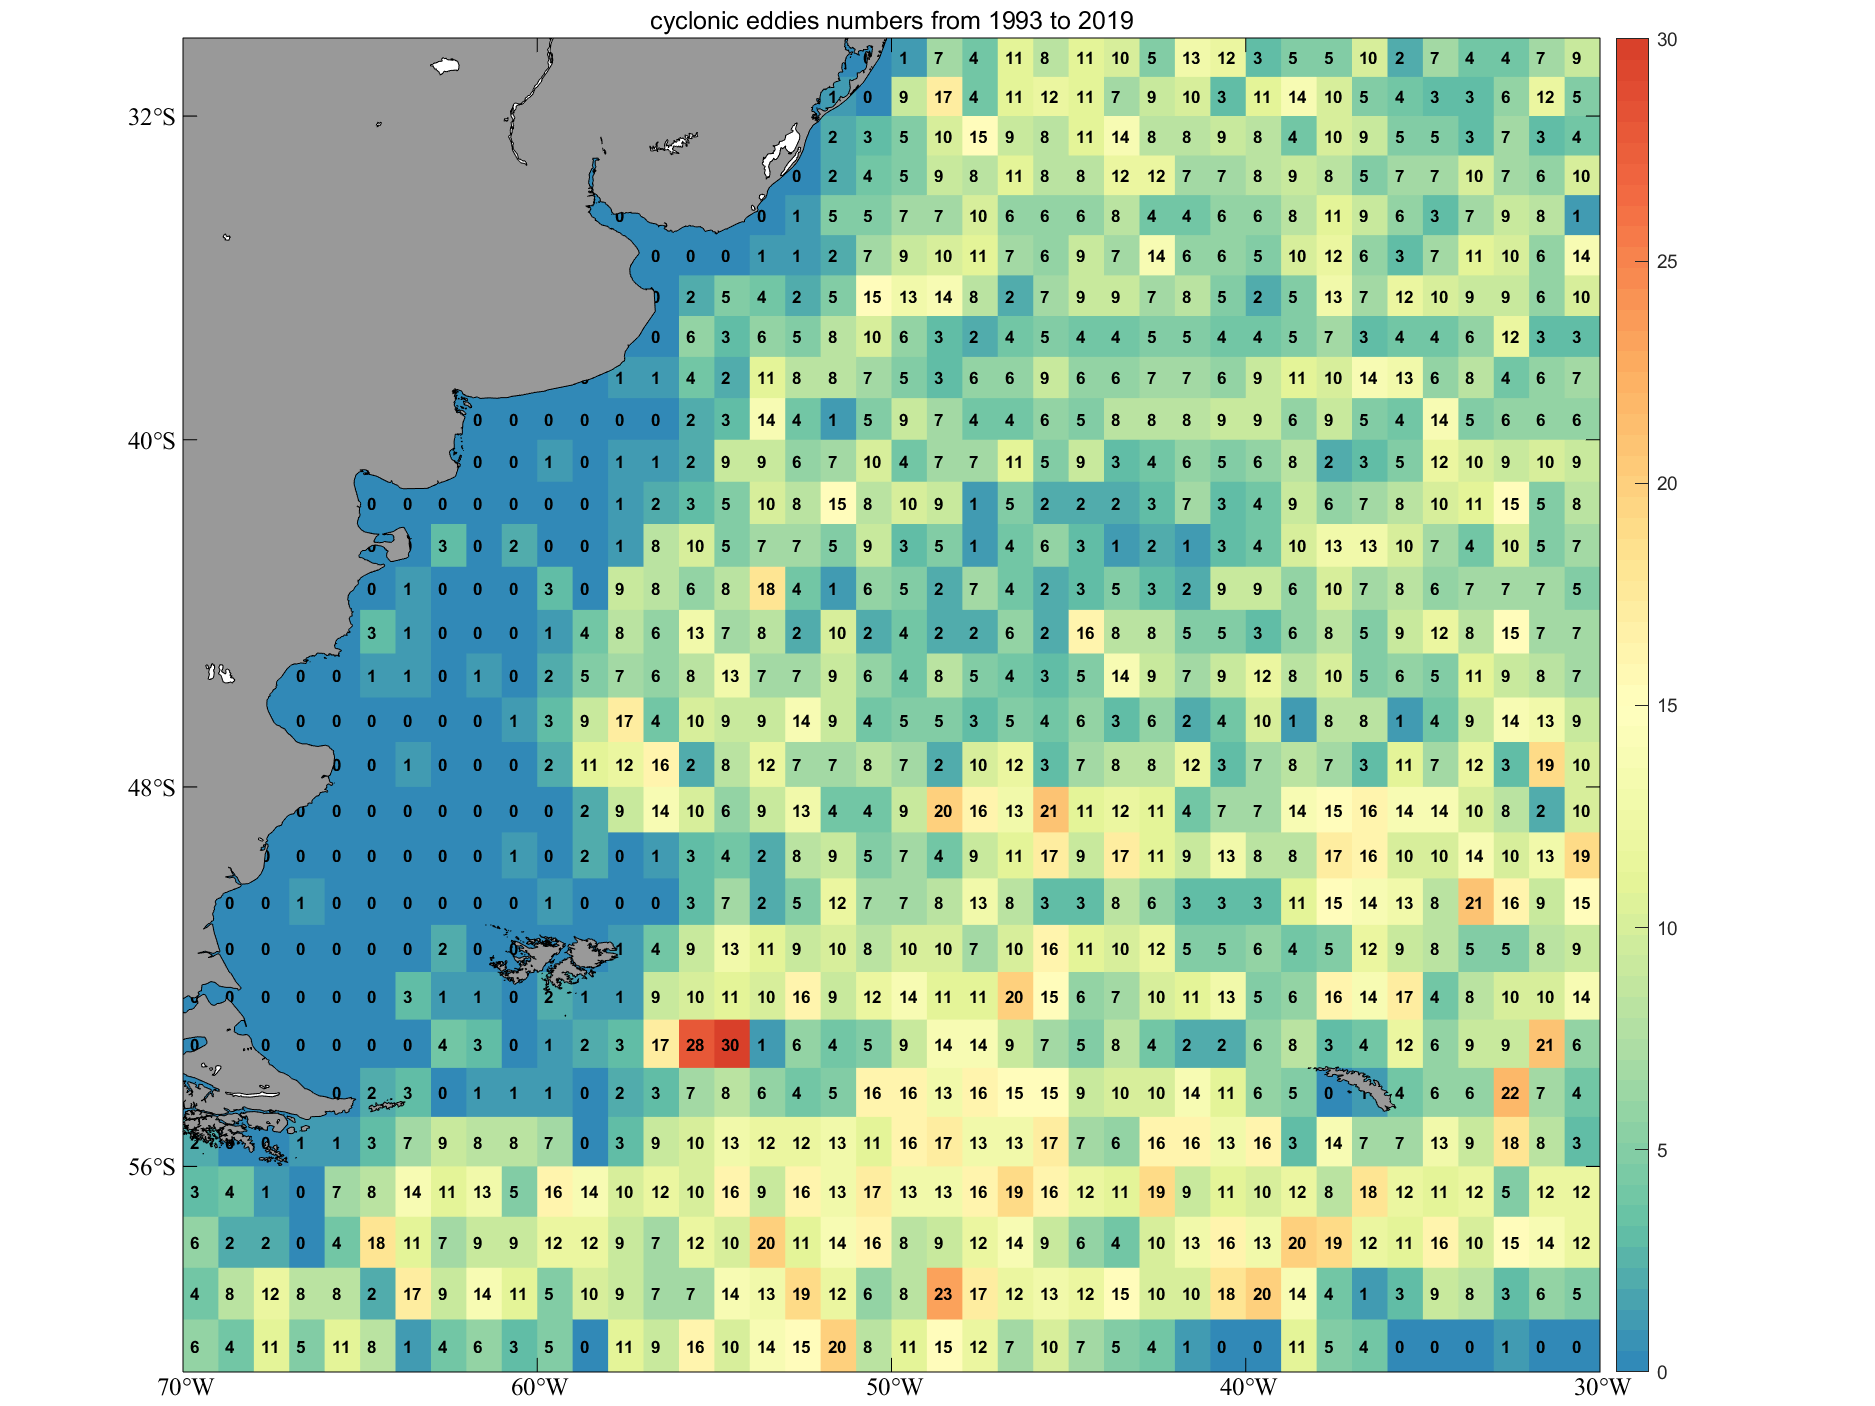
\includegraphics[width=15cm]{chapter/figure/cyclonic eddies numbers from 1993 to 2019.png}
  \caption
  {Cyclonic eddies numbers from 1993 to 2019}
  \label{cyclonic eddies numbers from 1993 to 2019}
\end{figure}

The following figures \ref{Anticyclonic eddies trajectories} and \ref{10 Cyclonic eddies trajectories} are the trajectories map of anticyclonic eddies and cyclonic eddies with lifetimes longer than 30 days. In order not to overlap the trajectories with each other, only one-tenth of the total eddies are selected and plotted on the map.


\begin{figure}[ht]
  \centering
  \setlength{\abovecaptionskip}{0.cm}
  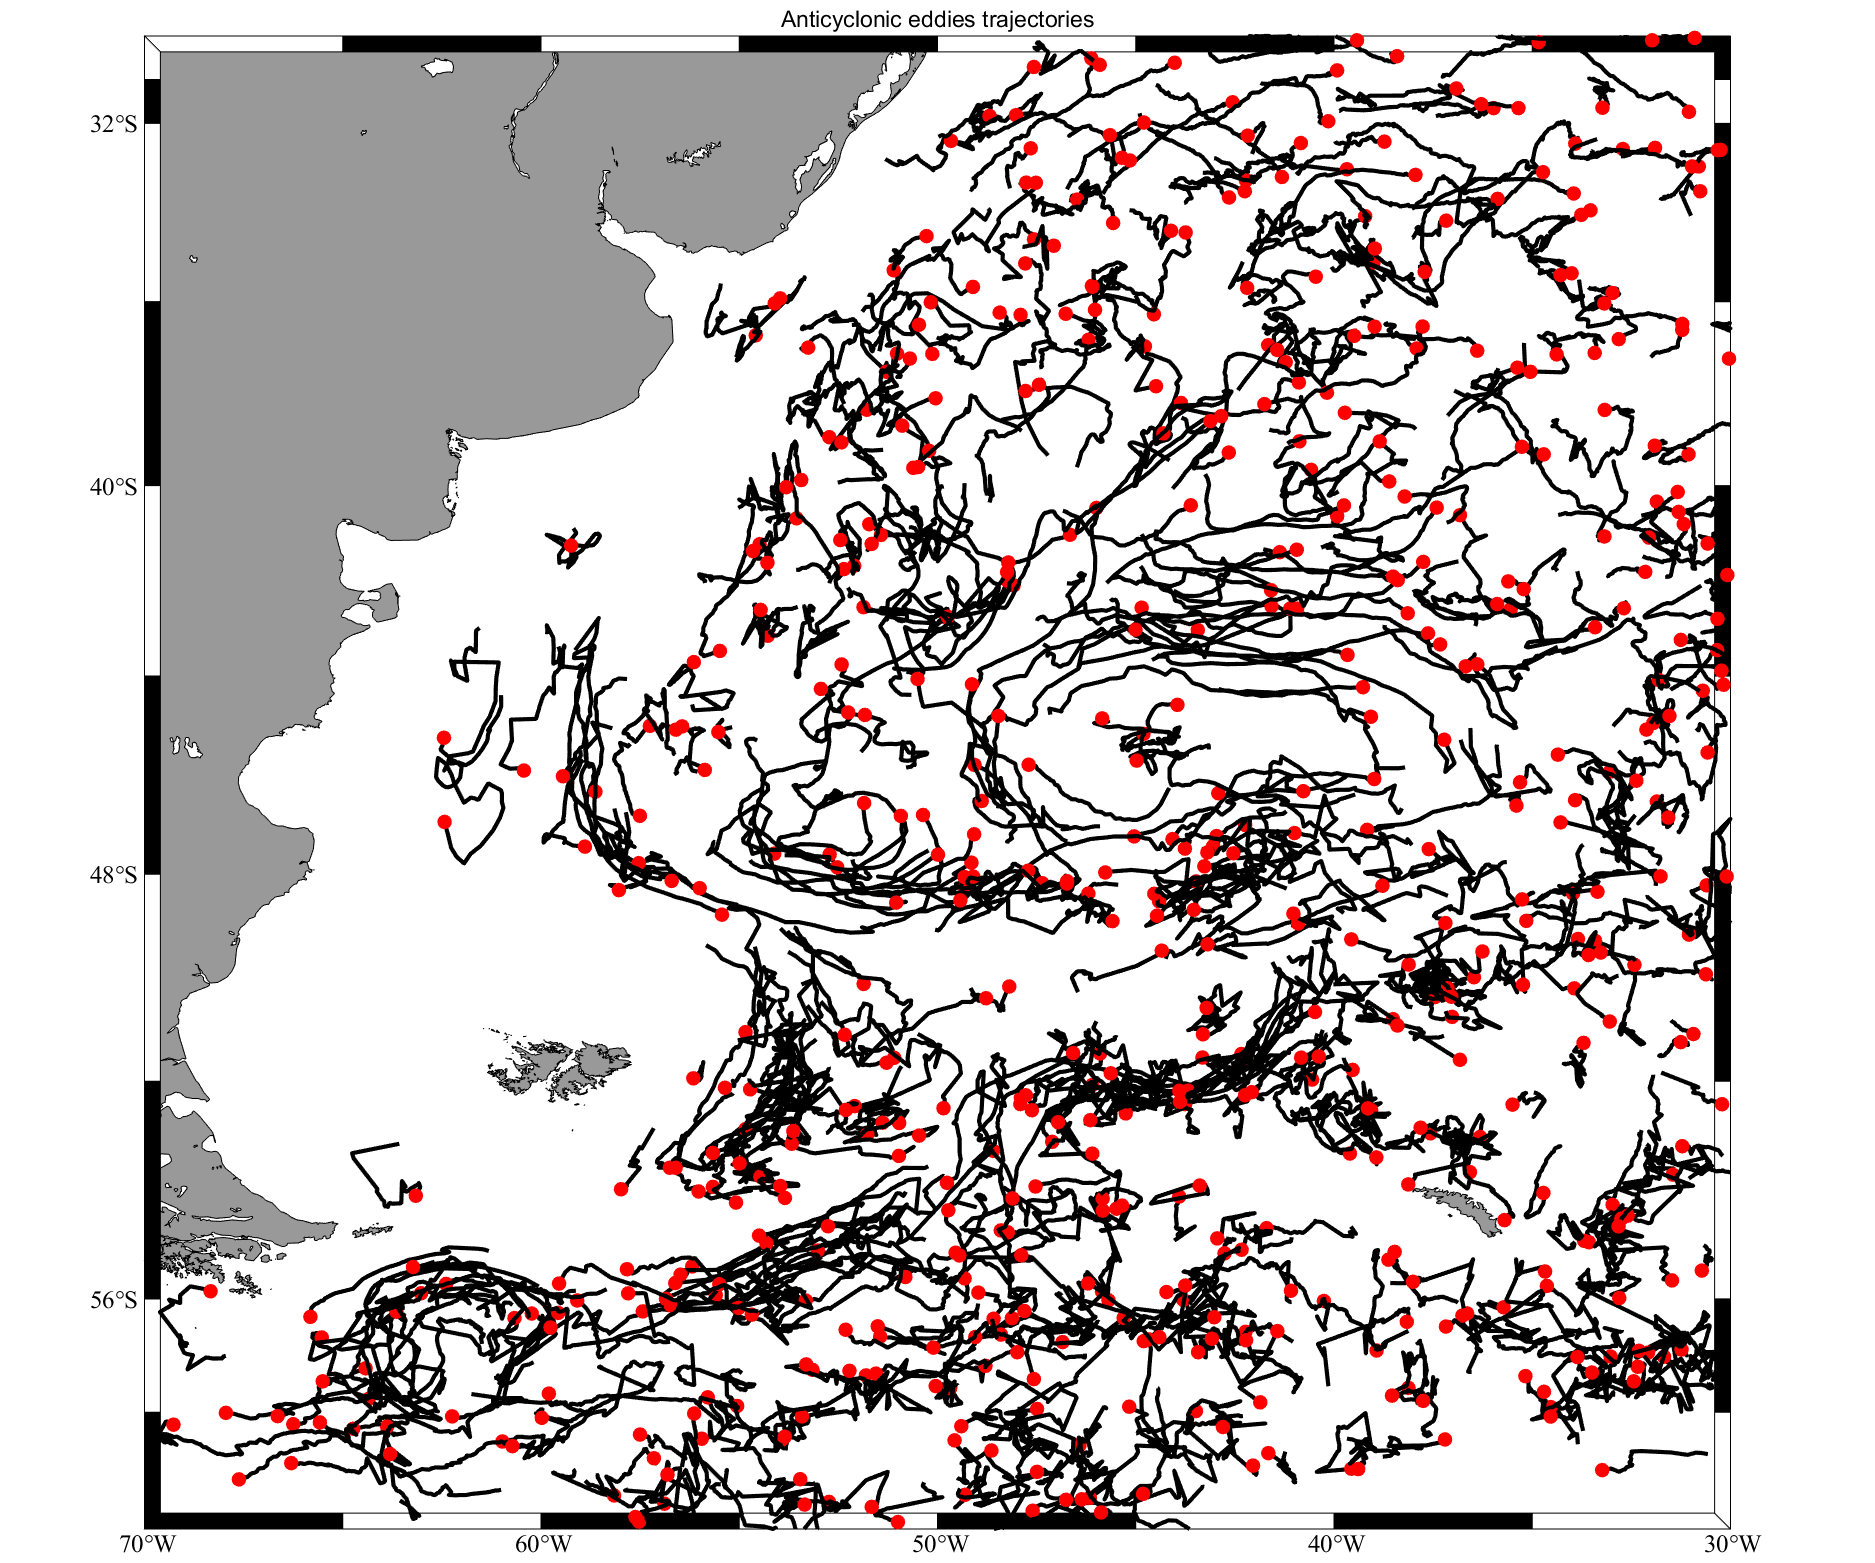
\includegraphics[width=1.0\textwidth]{chapter/figure/10 Anticyclonic eddies trajectories.png}
  \caption
  {Anticyclonic eddies trajectories from 1993-2018}
  \label{Anticyclonic eddies trajectories}
\end{figure}

\begin{figure}[ht]
  \centering
  \setlength{\abovecaptionskip}{0.cm}
  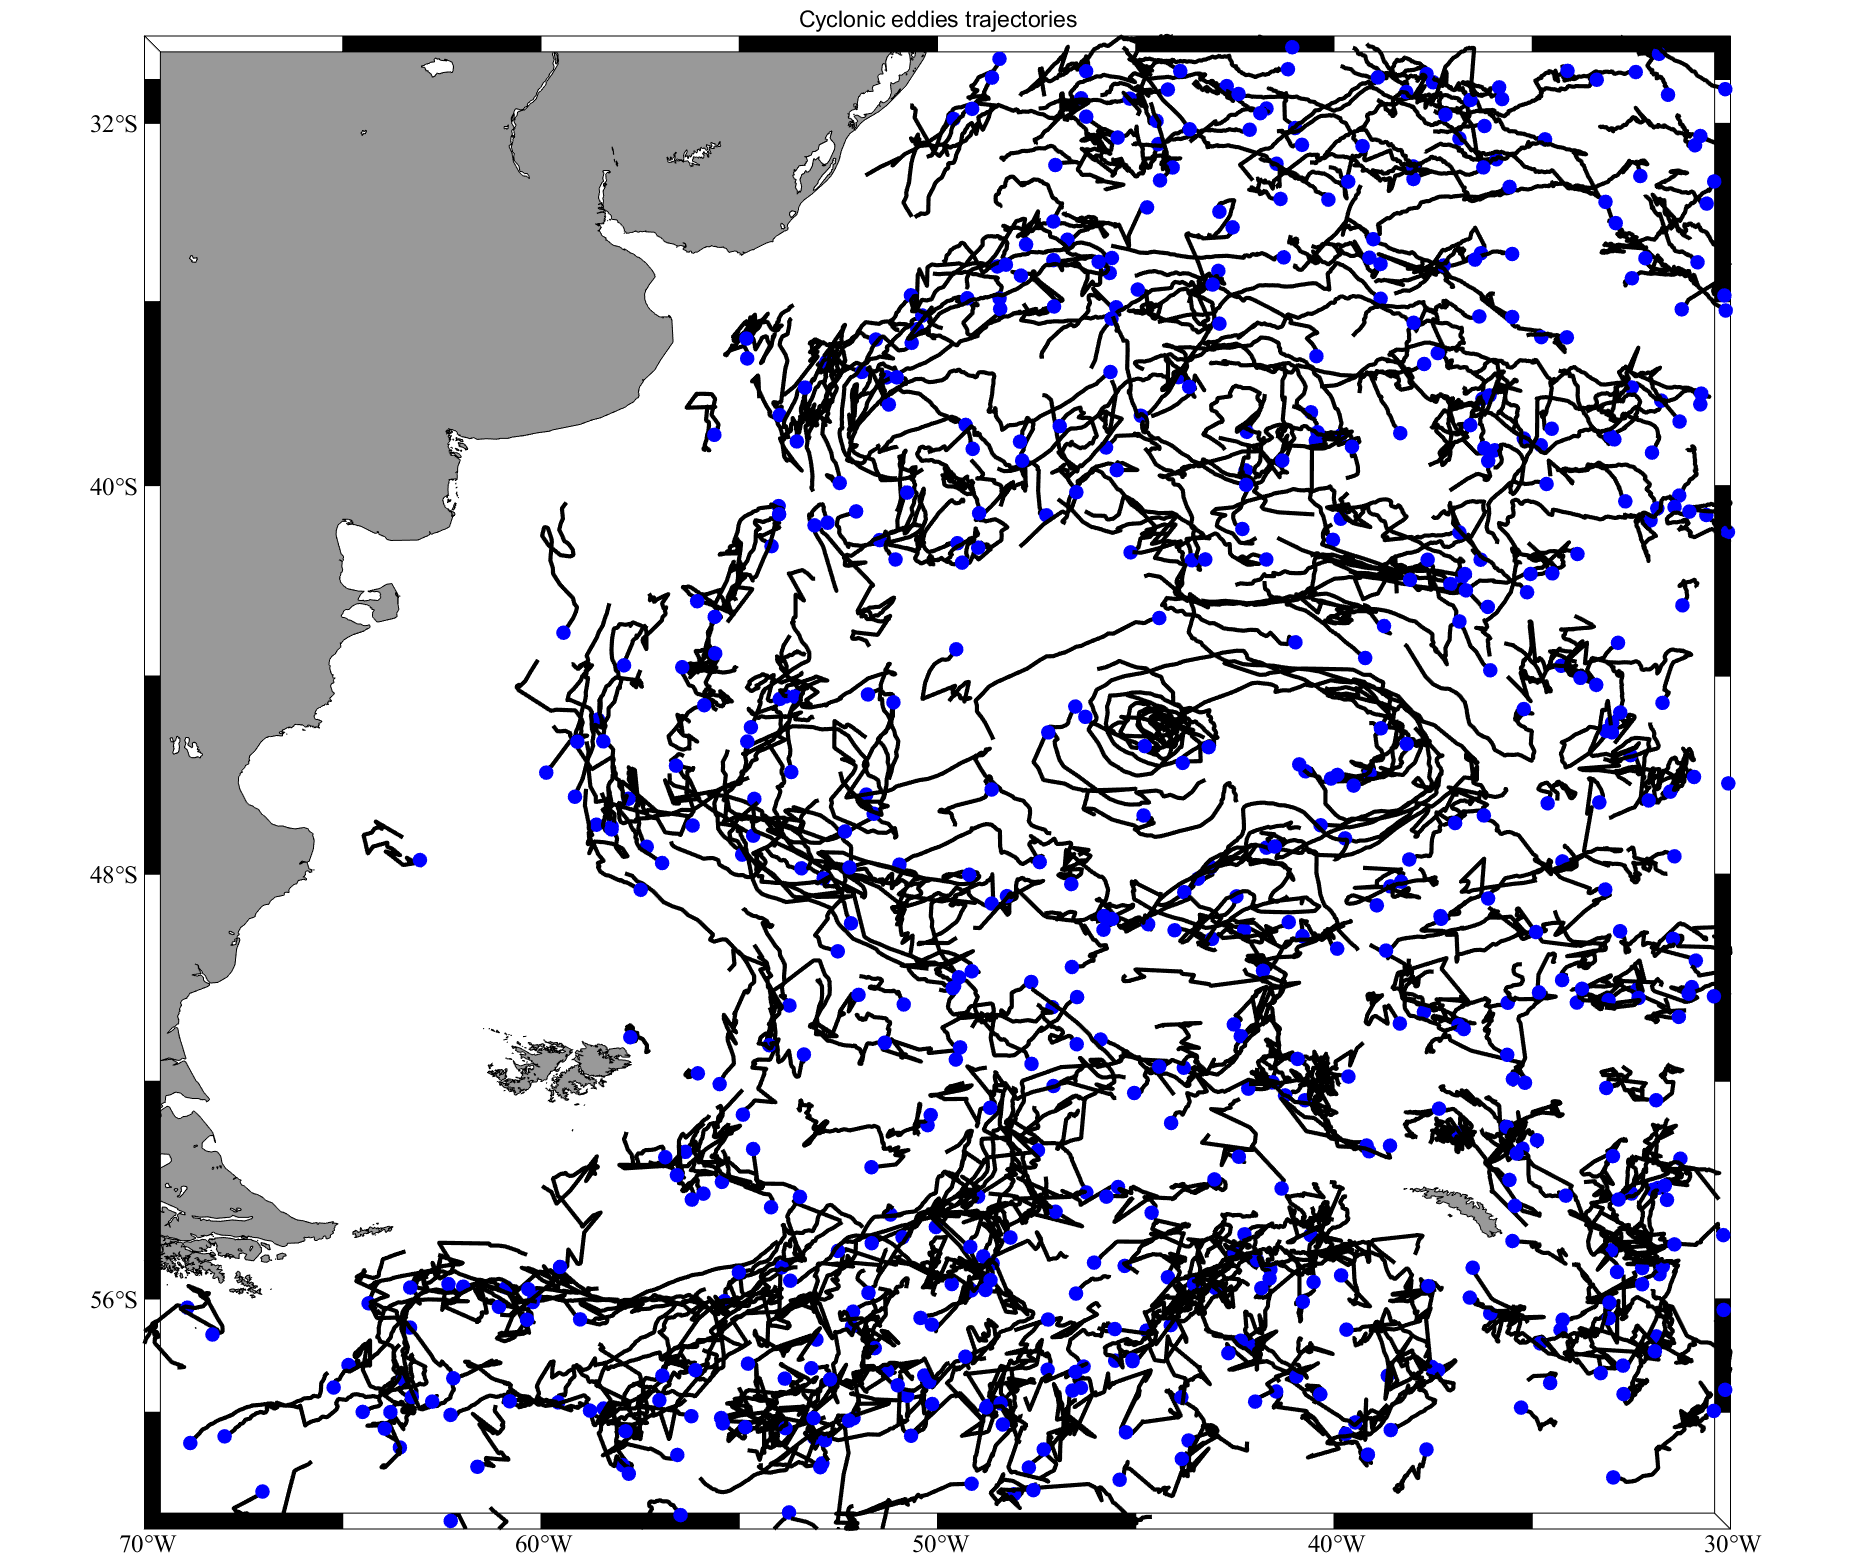
\includegraphics[width=1.0\textwidth]{chapter/figure/10 Cyclonic eddies trajectories.png}
  \caption
  {Cyclonic eddies trajectories from 1993-2018}
  \label{10 Cyclonic eddies trajectories}
\end{figure}


From figure \ref{Eulerian eddy number} , the observed temporal distribution of Eulerian eddies suggests that about 200-300 eddies would be generated in the Argentine Basin each year and the number of eddies decreases a little bit in recent years.
Eddies number distributes unevenly in the four-season: in summer, more eddies would appear and fewer eddies would be generated in winter. This pattern is similar to the results found in chapter \ref{Eddies features analysis}. The number of cyclonic eddies outweighs that of anticyclonic eddies by about 5\%.

The radius of Eulerian eddies is about 70 km, and anticyclonic eddies are a little bigger than cyclonic ones. The result is about twice as large as the Lagrangian eddy, which implies that Eulerian detection method may outweigh coherent transport carried by oceanic eddies and the outer part of Eulerian eddies was not so robust.

\begin{figure}[ht]
  \centering
  \setlength{\abovecaptionskip}{0.cm}
  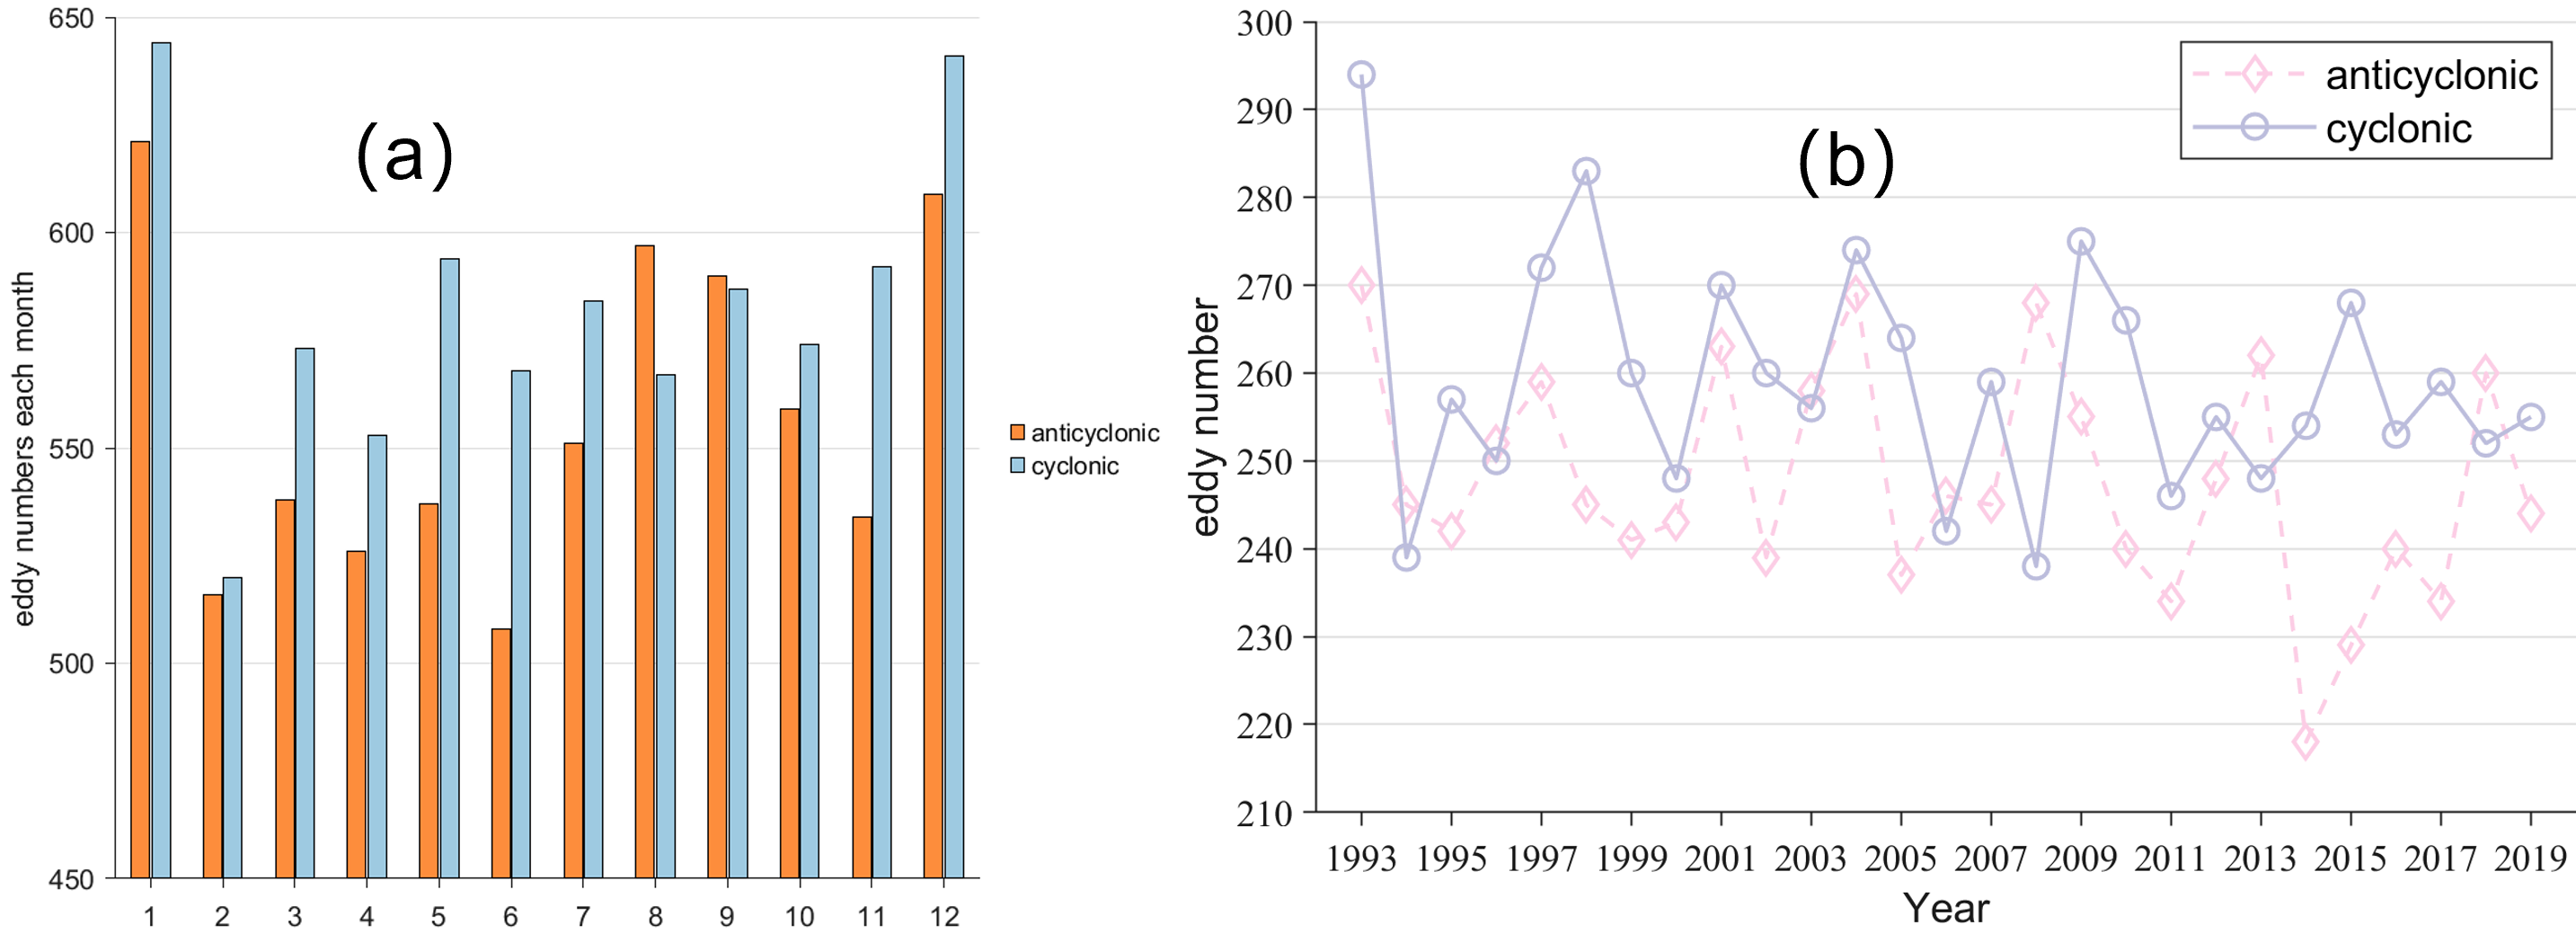
\includegraphics[width=15cm]{chapter/figure/Eulerian eddy number.png}
  \caption
  {Monthly and annual volume change characteristics of Eulerian eddy}
  \label{Eulerian eddy number}
\end{figure}


\begin{figure}[ht]
  \centering
  \setlength{\abovecaptionskip}{0.cm}
  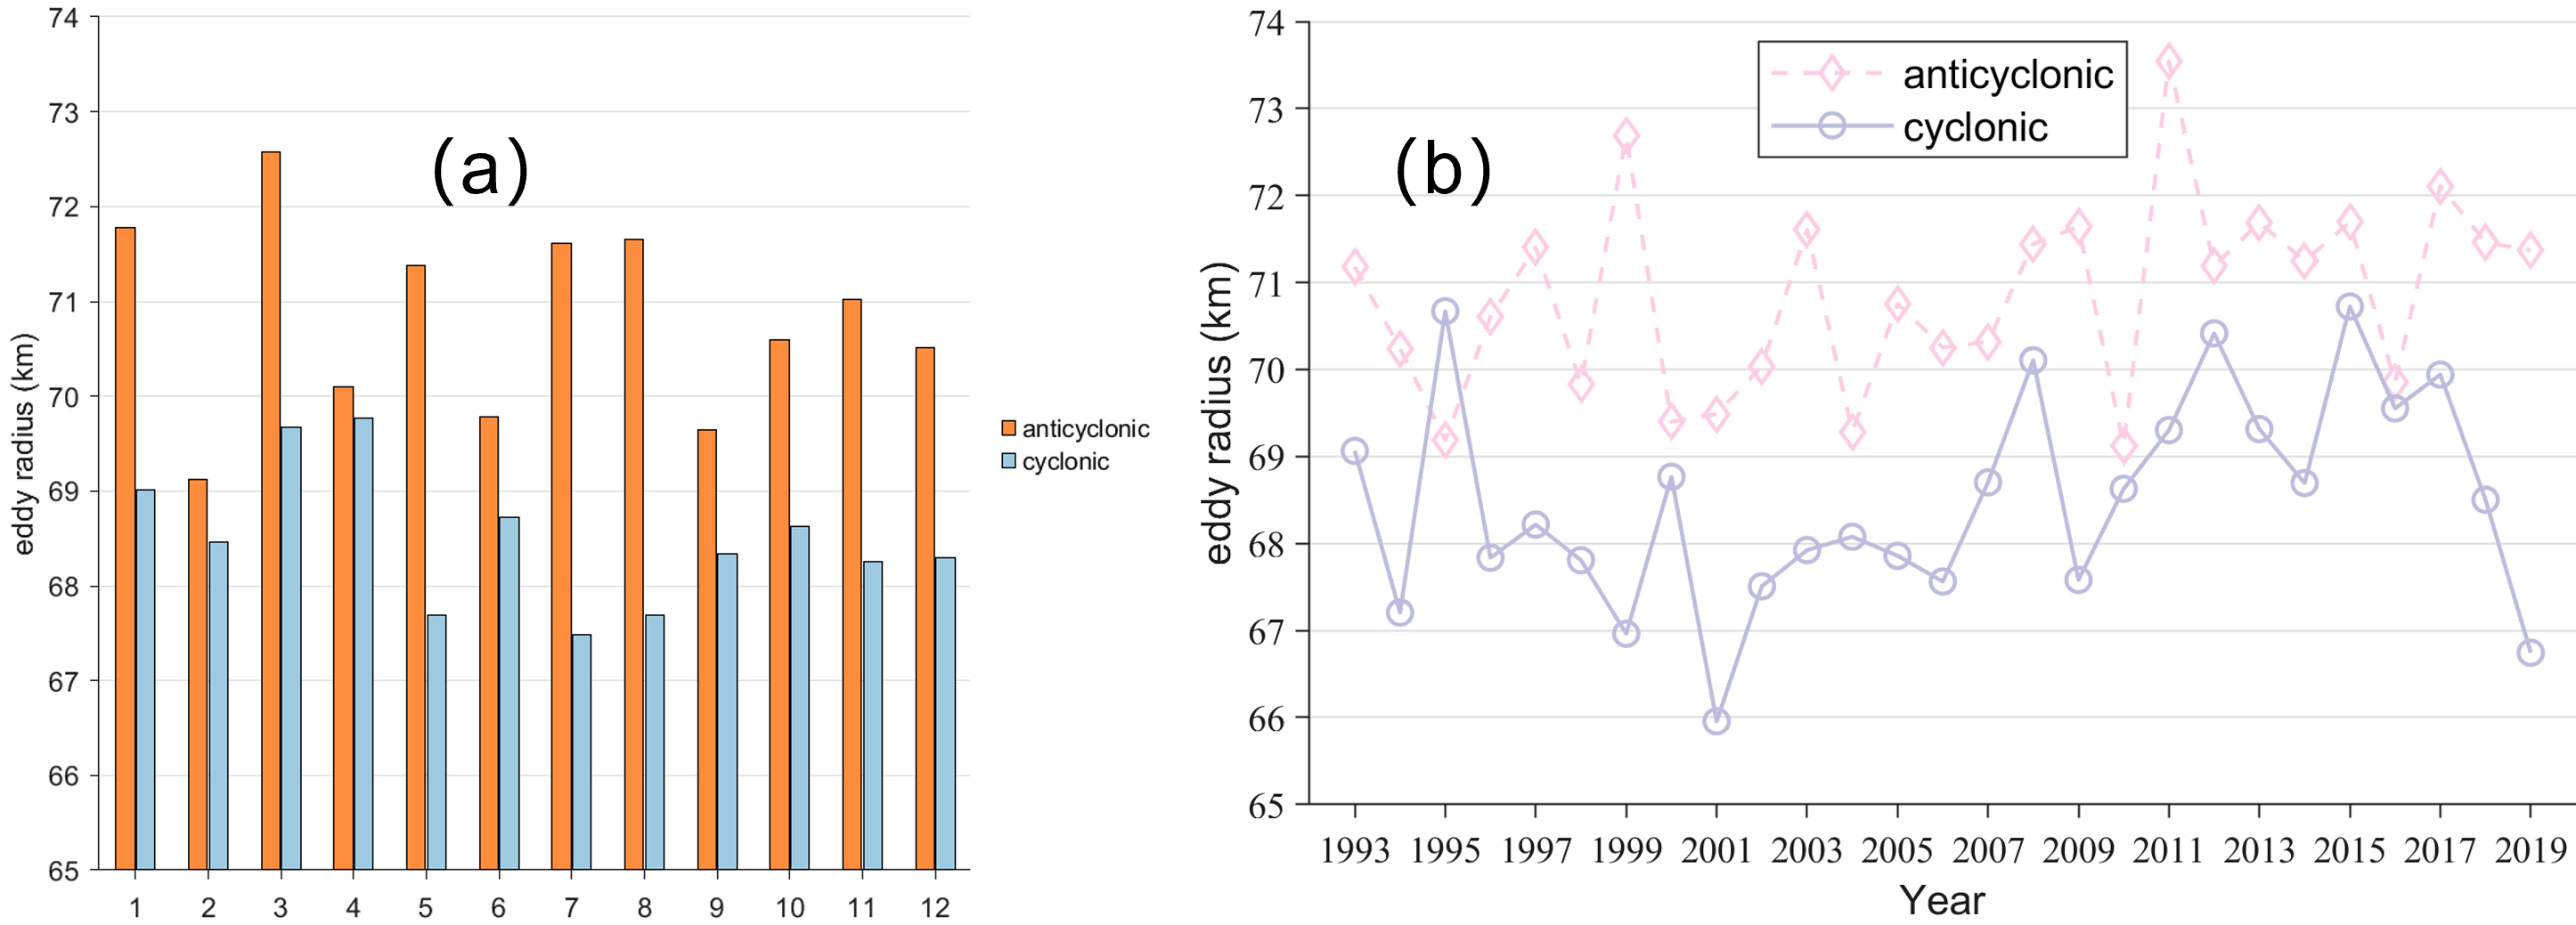
\includegraphics[width=15cm]{chapter/figure/Eulerian eddy radius.png}
  \caption
  {Seasonal and annual variation of Eulerian eddy number and radius}
  \label{Eulerian eddy radius}
\end{figure}


Figure \ref{Cyclonic eddy lifetime Frequency} and \ref{Anticyclonic eddy lifetime Frequency}
show the life estimation of Eulerian eddies, eddies with life estimation ranging from 30 to 60 days occupies 61\% of the entire number of vortexes while eddies with lifetime shorter than 30 days only account for 8\% and eddies with life-range over 180 days only takes up 1.5\% (1.6\% in cyclonic eddies and 1.4\% in anticyclonic eddies). The most long-living eddy lasted for 308 days. Thus, choosing 30 days as the coherent time for LAVD methods is convincing. 

\begin{figure}[ht]
  \centering
  \setlength{\abovecaptionskip}{0.cm}
  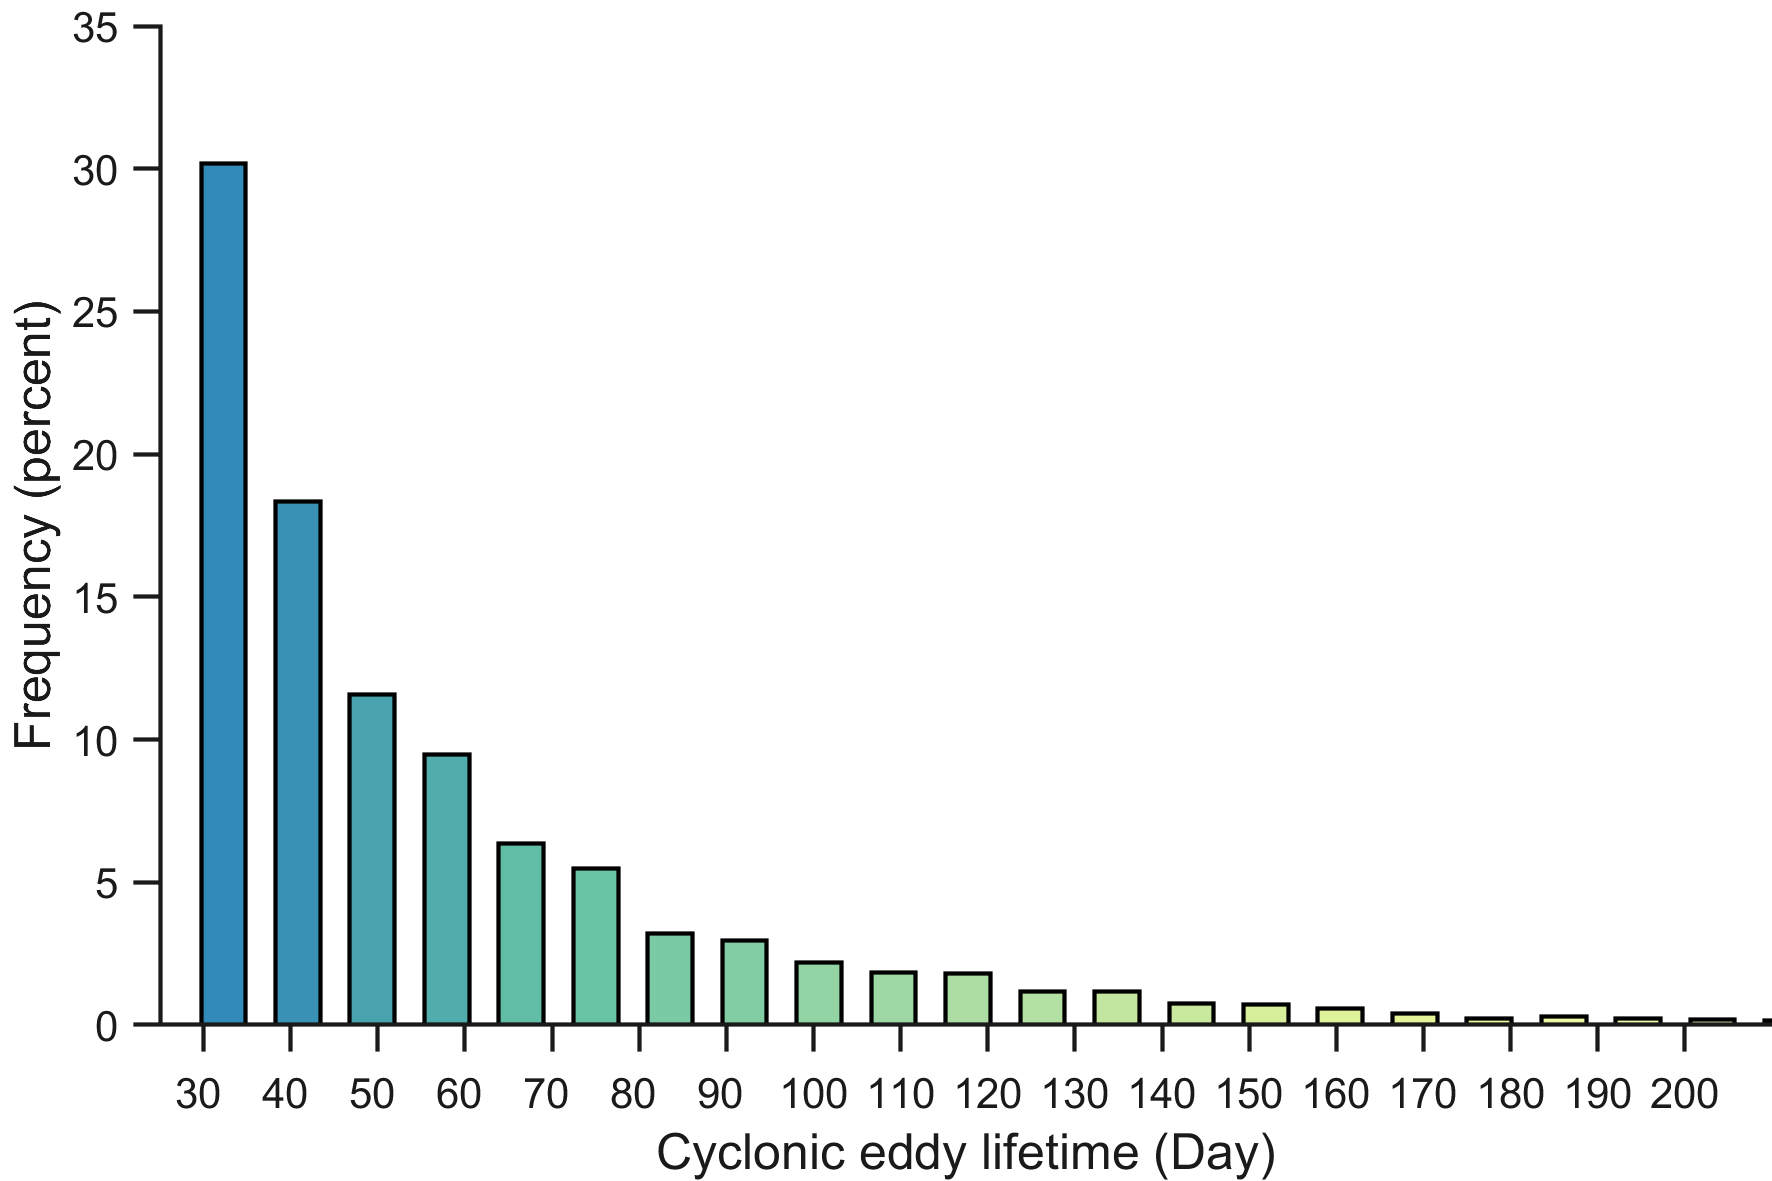
\includegraphics[width=15cm]{chapter/figure/Cyclonic eddy lifetime Frequency.png}
  \caption
  {Cyclonic Eulerian eddy lifetime Frequency}
  \label{Cyclonic eddy lifetime Frequency}
\end{figure}

\begin{figure}[ht]
  \centering
  \setlength{\abovecaptionskip}{0.cm}
  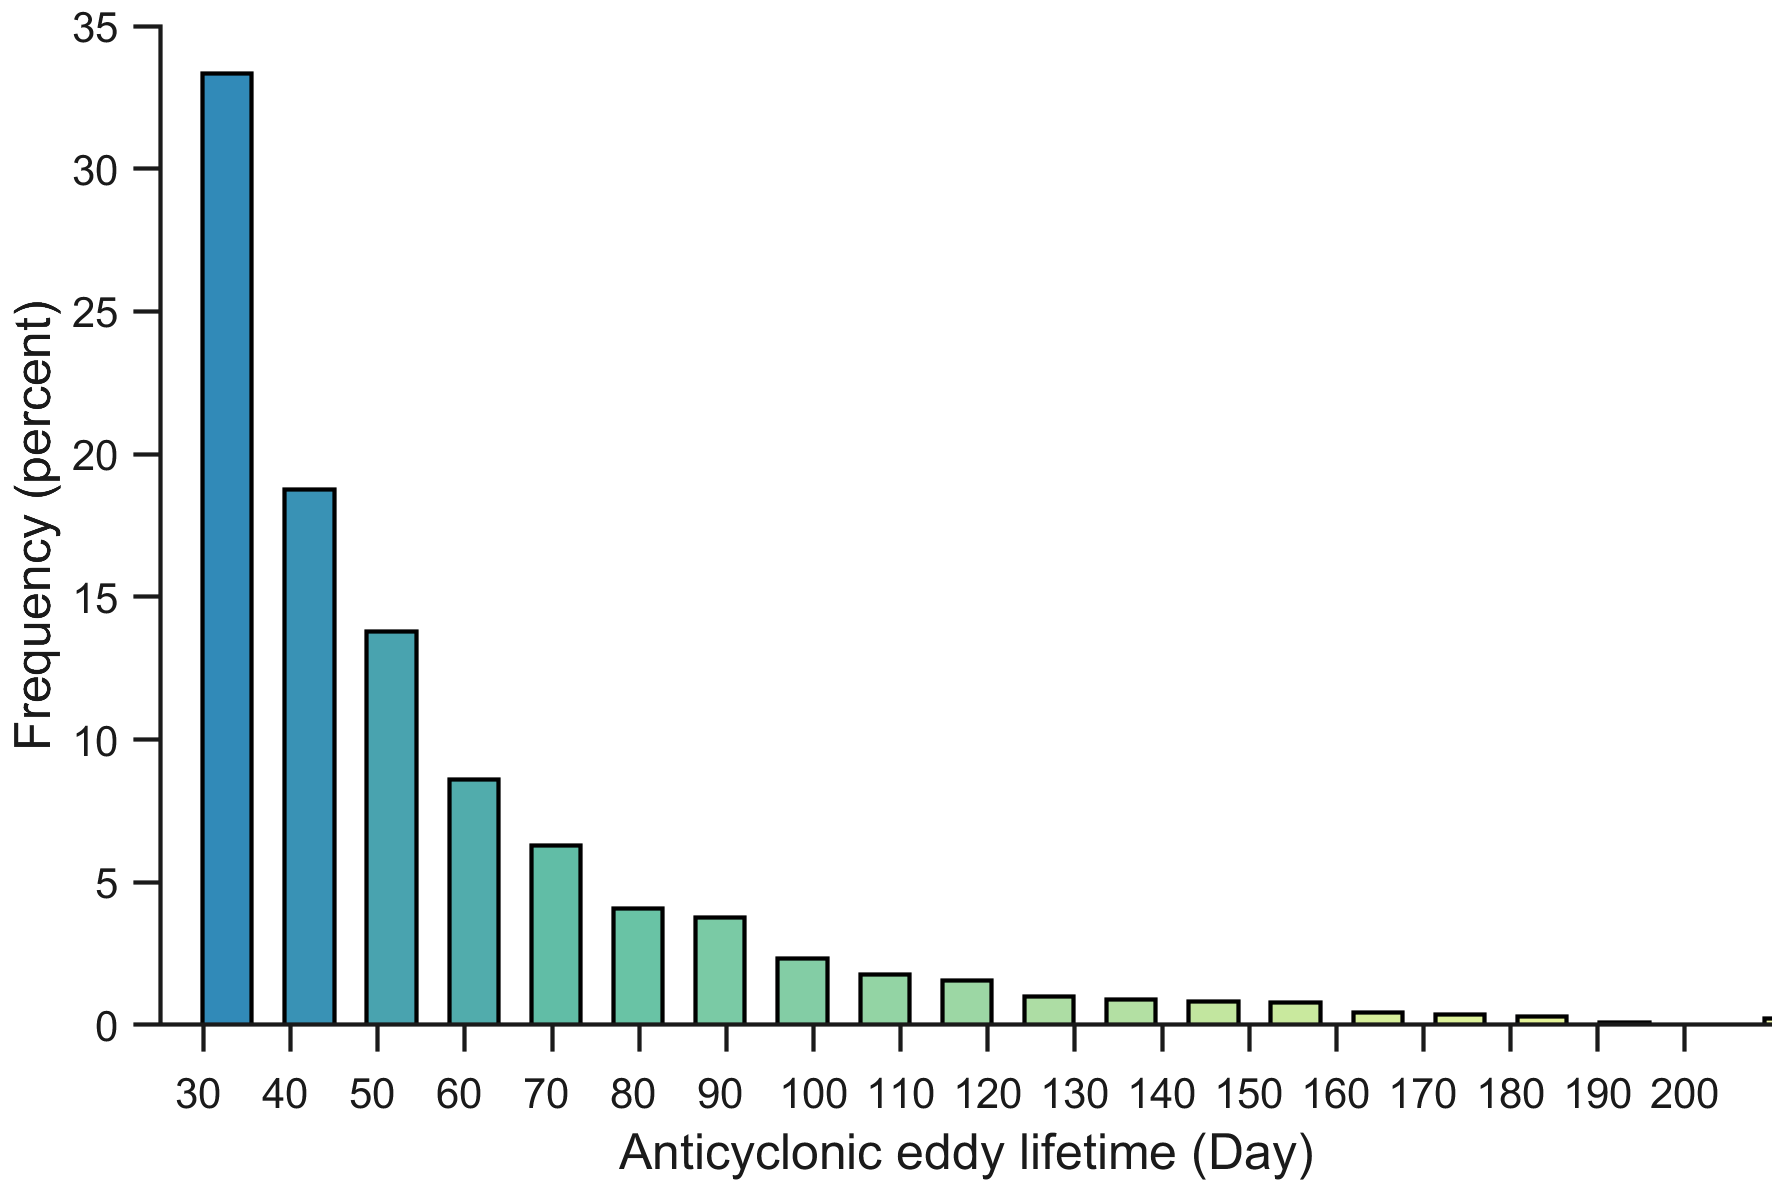
\includegraphics[width=15cm]{chapter/figure/Anticyclonic eddy lifetime Frequency.png}
  \caption
  {Anticyclonic Eulerian eddy lifetime Frequency}
  \label{Anticyclonic eddy lifetime Frequency}
\end{figure}

\section{Comparison of Lagrangian and Eulerian methods}

Since we adopt different methods to detect eddies, it is necessary to test the robustness of the results.


Search through the whole eddies dataset, we have found an Eulerian eddy that originated from 04-Aug-2006 and lasted for 140 days and the corresponding Lagrangian eddy has $t_0 = 2014-09-01$ and a coherent time of 120 days.

Figure \ref{coherence of eddy} shows the evolution process of this selected vortex (x label represents the lontitude and y label represents the latitude). In the figure, the coherent Lagrangian eddy part is marked in red, the blue dots represent the area enclosed by the Eulerian eddy, and the black ring shows the particle outside of the Eulerian eddy. We release the particles and find that the Eulerian eddy could maintain the overall shape in the first 15 days and then the outer part of the Eulerian eddy would deform and stretch in the evolution process. After 70 days, two fluid arms are flung from the core of the Euler vortex and 100 days later, only part of the blue particle is still inside the Eulerian vortex. However, the LAVD Lagrangian eddy still maintains the main body and tracks almost all of the particles inside although the shape of the vortex changes a little bit.

\begin{figure}[ht]
  \centering
  \setlength{\abovecaptionskip}{0.cm}
  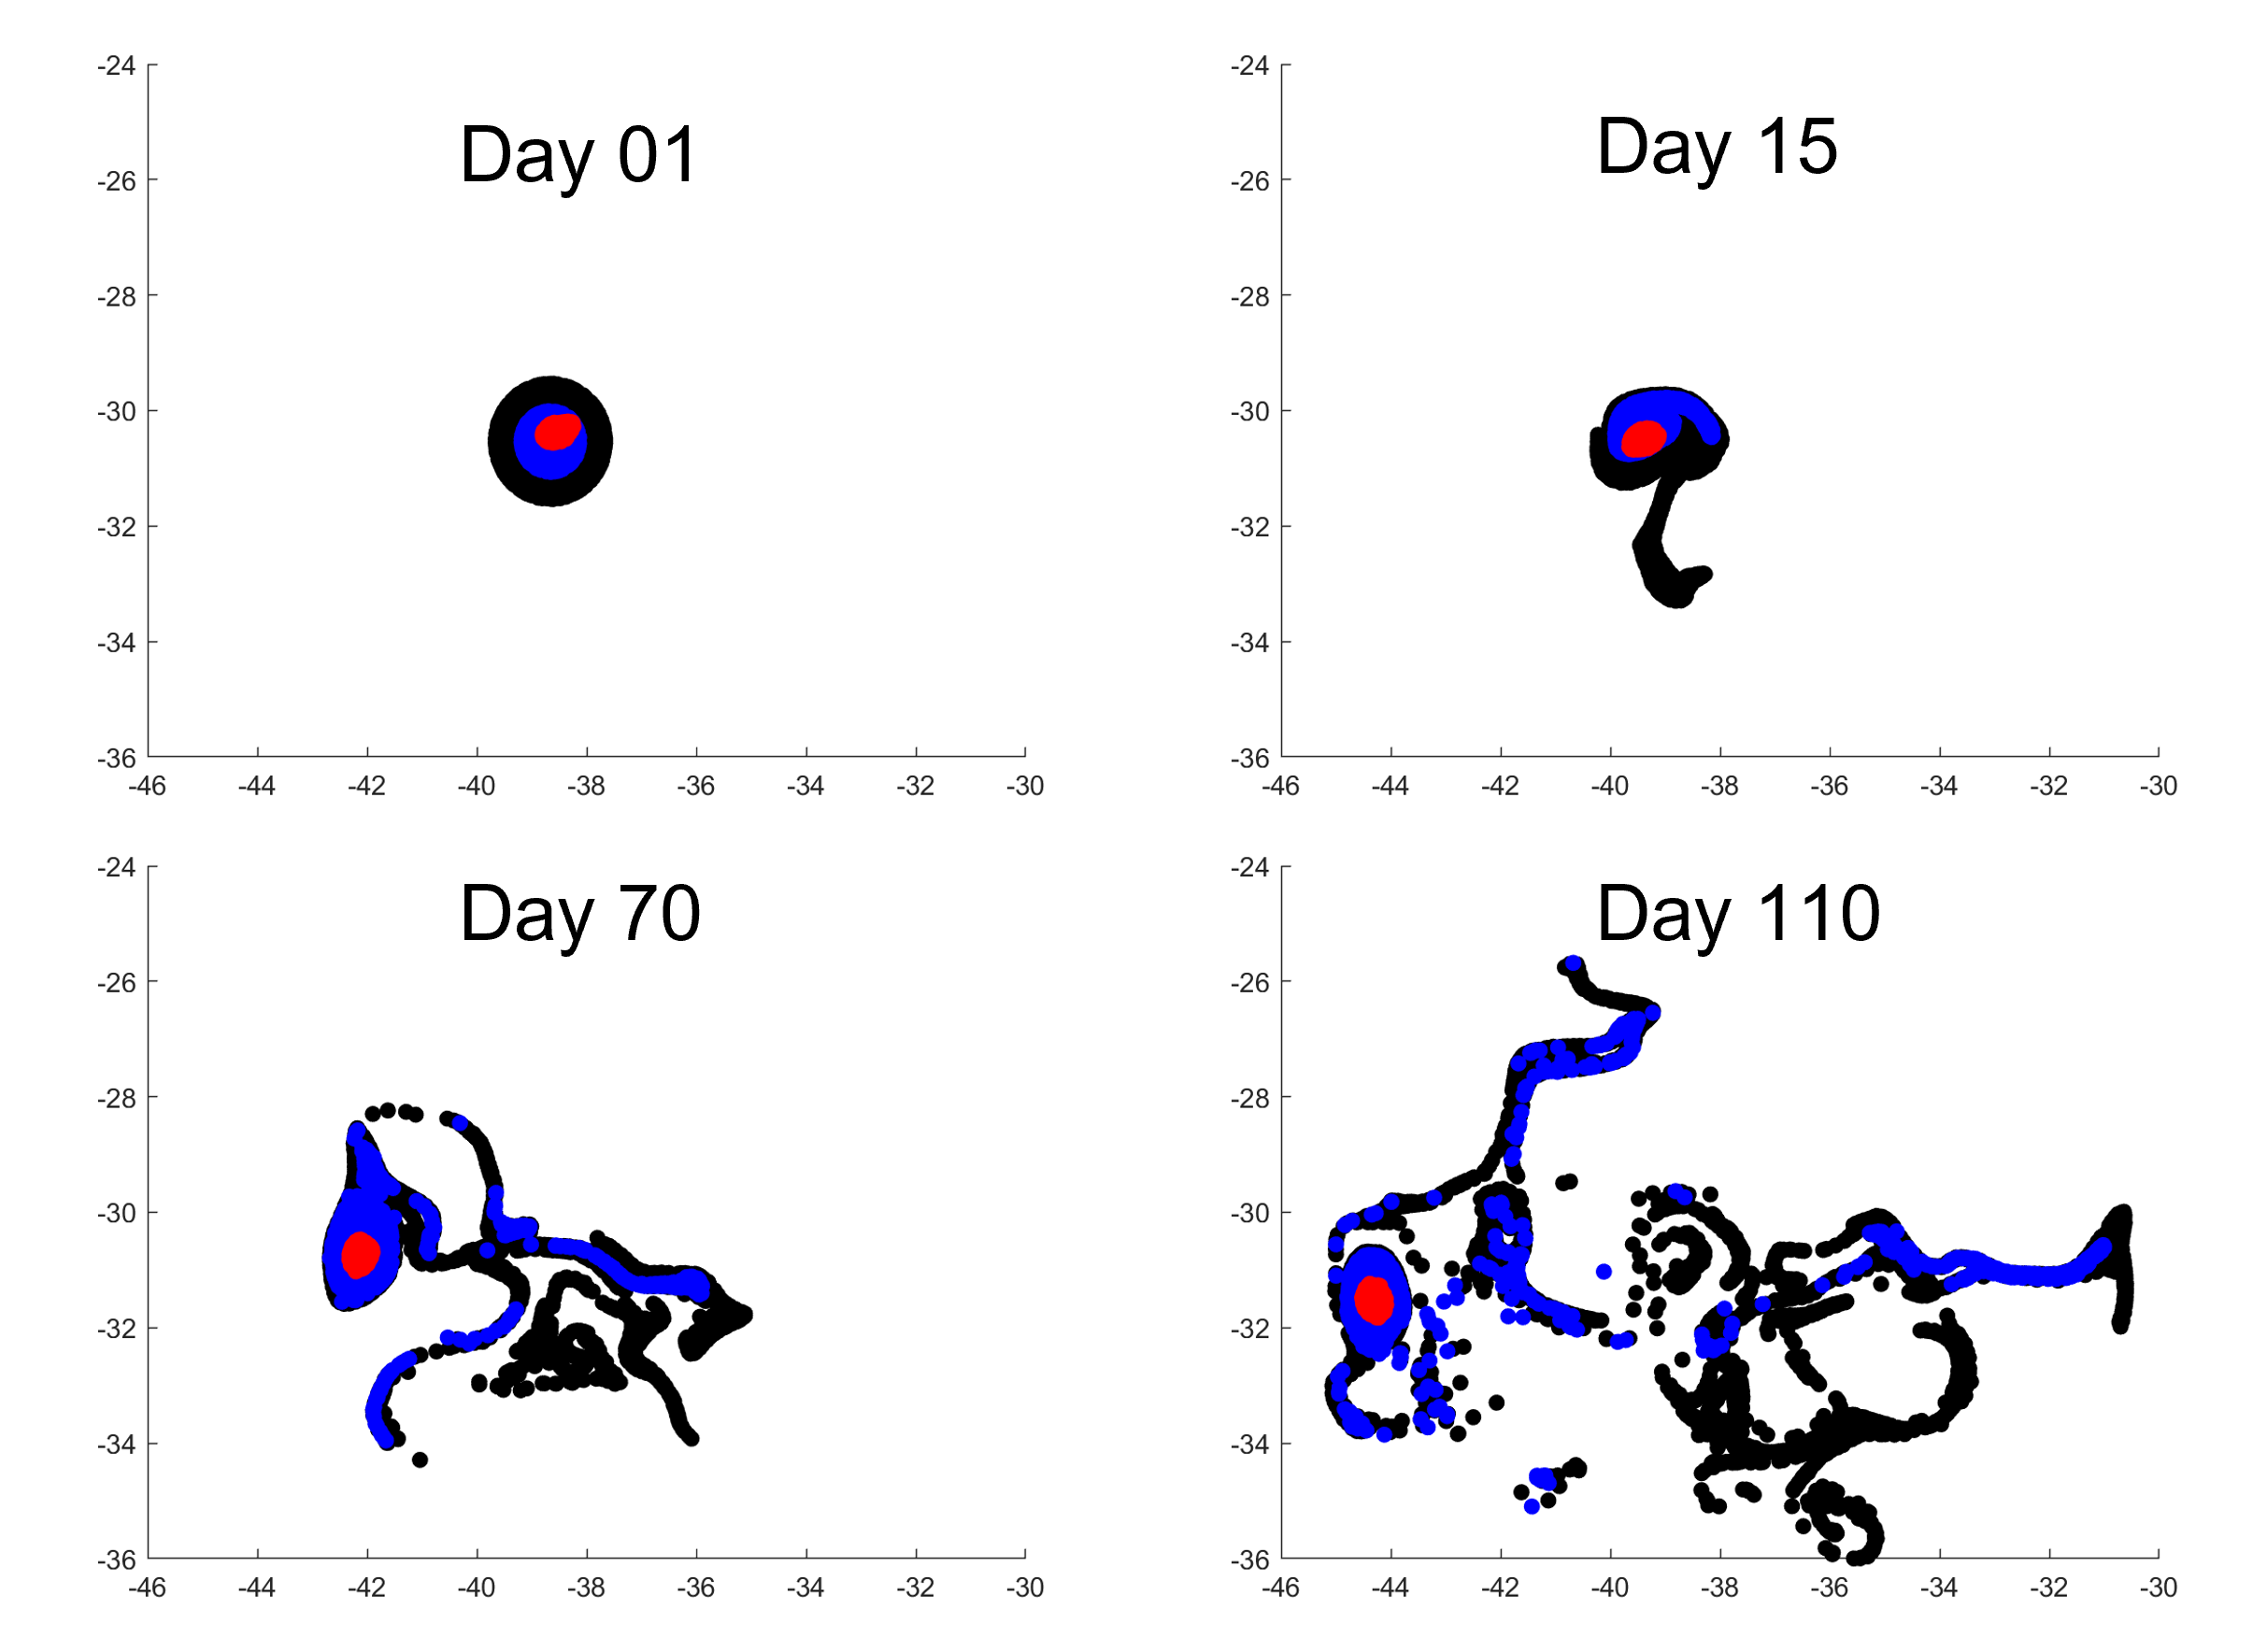
\includegraphics[width=1.0\textwidth]{chapter/figure/coherence of eddy.png}
  \caption
  {Evolution of one elected eddy}
  \label{coherence of eddy}
\end{figure}

Lagrangian eddies-detecting algorithms, thus, provide a convincing path to estimate eddies' number, size and carrying capacity for transporting a large amount of waters and particles both in oceanic model data and observational data.

\clearpage

\section{Conclusion}

In this chapter, we use SSHA Eulerian method to detect eddies in the same research area and research period. We have several findings as concluded below:

\begin{itemize}
  \item [1)] 
  The general appearance rules of the Eulerian eddy are quite the same as the Lagrangian eddy.
  \item [2)]
  Eulerian eddies tend to have a bigger size and the number of eddies counted using the Eulerian method outweighs the number in LAVD research.  

  \item [3)]
  A case study of one long-living eddy suggests the robustness of the Lagrangian coherent eddy's  transport capacity.

  \item[4)]
  30 days may be a reasonable choice for the detection period for oceanic eddy. 
\end{itemize}


\newpage

